\documentclass[12pt]{article}

% Allow block comment commands
\usepackage{comment}

\begin{comment}
draft - disables image rendering, shows black boxes at hyphenation issues

Defaults:
	10pt
	notitlepage
	a4paper (usletter on some distros)
	singleside (twoside changes the margins for a binding)

Style:
http://practicaltypography.com
https://www.sharelatex.com/learn/Paragraphs_and_new_lines

title styling
http://texblog.org/2012/07/03/fancy-latex-chapter-styles/

Left-aligned text; equal spacing between words, better readability
	May look "unprofessional", books, articles typically use fully justified
	ragged2e retains hyphenation and attempts to give a more uniform right edge, but maintains equal spacing between words
\end{comment}
\usepackage[document]{ragged2e}
% Adjust default length before hyphenation, reducing amount of hyphenation
\setlength{\RaggedRightRightskip}{0pt plus 3.5em}
\raggedright


% Single space after a full stop, modern typographic readability standard
\frenchspacing

% Paragraph spacing with no indent; breaks up huge blocks of text
\usepackage{parskip}

% Line spacing (Default or slightly larger?)
\usepackage{setspace}
%\onehalfspacing

% Header and footer
\usepackage{fancyhdr}
\fancyhead[L]{\nouppercase{\textbf{\rightmark}}}
\fancyhead[R]{\textbf{\thepage}}
\cfoot{}
\renewcommand{\headrulewidth}{0.5pt}
%\renewcommand{\footrulewidth}{0.5pt}
%textsf ?

% Roman section numbering, numbered subsections
\renewcommand \thesection{\Roman{section}}
\renewcommand \thesubsection{\arabic{section}.\arabic{subsection}}

% Page decorations
% Adapted from: http://tex.stackexchange.com/questions/85904/showcase-of-beautiful-title-page-done-in-tex

\usepackage{tikz}

% Right side decorations
\newcommand\pagedecorationright{
\begin{tikzpicture}[remember picture,overlay,shorten >= -10pt]

\coordinate (aux1) at ([yshift=-15pt]current page.north east);
\coordinate (aux2) at ([yshift=-410pt]current page.north east);
\coordinate (aux3) at ([xshift=-4.5cm]current page.north east);
\coordinate (aux4) at ([yshift=-150pt]current page.north east);

\begin{scope}[pagecolour!40,line width=12pt,rounded corners=12pt]
\draw
  (aux1) -- coordinate (a)
  ++(225:5) --
  ++(-45:5.1) coordinate (b);
\draw[shorten <= -10pt]
  (aux3) --
  (a) --
  (aux1);
\draw[opacity=0.6,pagecolour,shorten <= -10pt]
  (b) --
  ++(225:2.2) --
  ++(-45:2.2);
\end{scope}
\draw[pagecolour,line width=8pt,rounded corners=8pt,shorten <= -10pt]
  (aux4) --
  ++(225:0.8) --
  ++(-45:0.8);
\begin{scope}[pagecolour!70,line width=6pt,rounded corners=8pt]
\draw[shorten <= -10pt]
  (aux2) --
  ++(225:3) coordinate[pos=0.45] (c) --
  ++(-45:3.1);
\draw
  (aux2) --
  (c) --
  ++(135:2.5) --
  ++(45:2.5) --
  ++(-45:2.5) coordinate[pos=0.3] (d);   
\draw 
  (d) -- +(45:1);
\end{scope}
\end{tikzpicture}
}

% Left side decorations
\newcommand\pagedecorationleft{
\begin{tikzpicture}[remember picture,overlay,shorten >= -10pt]
\coordinate (aux1) at ([yshift=-15pt]current page.north west);
\coordinate (aux2) at ([yshift=-410pt]current page.north west);
\coordinate (aux3) at ([xshift= 4.5cm]current page.north west);
\coordinate (aux4) at ([yshift=-150pt]current page.north west);

\begin{scope}[pagecolour!40,line width=12pt,rounded corners=12pt]
\draw
  (aux1) -- coordinate (a)
  ++(-45:5) --
  ++(-135:5.1) coordinate (b);
\draw[shorten <= -10pt]
  (aux3) --
  (a) --
  (aux1);
\draw[opacity=0.6,pagecolour,shorten <= -10pt]
  (b) --
  ++(-45:2.2) --
  ++(-135:2.2);
\end{scope}
\draw[pagecolour,line width=8pt,rounded corners=8pt,shorten <= -10pt]
  (aux4) --
  ++(-45:0.8) --
  ++(-135:0.8);
\begin{scope}[pagecolour!70,line width=6pt,rounded corners=8pt]
\draw[shorten <= -10pt]
  (aux2) --
  ++(-45:3) coordinate[pos=0.135] (c) --
  ++(-135:3.1);
\draw
  (aux2) --
  (c) --
  ++(45:2.5) --
  ++(135:2.5) --
  ++(-135:2.5) coordinate[pos=0.3] (d);   
\draw 
  (d) -- +(135:1);
\end{scope}
\end{tikzpicture}
}
\definecolor{pagecolour}{cmyk}{1,.60,0,.40}

% Font choices - LaTeX default is computer modern, a bit thin for my liking
% https://www.tug.org/mactex/fonts/LaTeX_Preamble-Font_Choices.html
% Palatino body text
%\renewcommand{\rmdefault}{ppl}
%\linespread{1.05}

% Tools
\usepackage{mathtools}
\usepackage{graphicx}
\usepackage{epstopdf}
\usepackage{siunitx}
\usepackage{acronym}
\usepackage{hyperref}
% In text subscripts and superscripts
\usepackage{fixltx2e}
% Side captioned figures
\usepackage{sidecap}

% Some handy commands for referencing (copied from old template)
\newcommand{\figref}[2][\figurename~]{#1\ref{#2}}
\newcommand{\tabref}[2][\tablename~]{#1\ref{#2}}
\newcommand{\secref}[2][Section~]{#1\ref{#2}}
\renewcommand{\vec}[1]{\mathbf{#1}}

\begin{comment}
Useful LaTeX commands/tools:
	\clearpage ends the current page and causes all figures and tables that have so far appeared in the input to be printed.
	www.doi2bib.org

General writing tips:
https://owl.english.purdue.edu/owl/section/1/2/
	3-5 sentences per paragraph; one idea, contrast, a break, balance
	15-20 words per sentence; comprehension lowers the longer it gets
	25-33 syllables; most like typical speech
	50-75 characters per line, ~65 seems optimal
	Use plain English; simpler words are better words
	Explain all technical jargon and abbreviations at first use

Science writing:
	Figure text and the abstract should be independent from main text
	List assumptions after each sub-theory (being clear about problems)
	Every review is gold dust, people can only read the first time once
	Send your draft to your references to see if you've cited their work fairly

\end{comment}

\begin{document}

%Front Matter

% Remove page numbering
\pagenumbering{garble}
\pagestyle{empty}

% Fancy title page, modified version of fancy-title.tex
\begin{titlepage}
\center
% Headings
\textsc{\huge University of Exeter}\\[1cm]
\textsc{\Large MPhys Project}\\[1.5cm]
%\textsc{\large Minor Heading}\\[0.5cm]

% Title
\rule{\linewidth}{0.5mm}\\[0.4cm]
\begin{doublespace}
{\LARGE \textbf{Thermoelectric Efficiency of Zero-dimensional Nanocomposites}}\\[0cm]
\end{doublespace}
\rule{\linewidth}{0.5mm}\\[2.5cm]
 
% Authors
\begin{minipage}{0.4\textwidth}
\begin{flushleft} \large
\emph{Author:}\\
Callum \textsc{Vincent}
\end{flushleft}
\end{minipage}
~
\begin{minipage}{0.4\textwidth}
\begin{flushright} \large
\emph{Supervisor:} \\
Prof. G. P. \textsc{Srivastava}
\end{flushright}
\end{minipage}\\[4cm]

% Date
{\large April 2015}

\pagedecorationleft
\pagedecorationright
\end{titlepage}

% Abstract page
\begin{center}
{\Huge\textbf{Abstract}}\\[2cm]
\end{center}
\begin{justify}
Thermoelectrics are currently limited by their heat to electric conversion efficiency. If their efficiency can be improved 3$\times$ then a wide array of technological applications can be developed. Nanocomposite structuring is a potential technique for achieving this. We utilise an effective medium approximation to calculate the thermoelectric efficiency of a zero-dimensional SiGe nanocomposite. We find that silicon spheres of 10nm diameter densely packed in a germanium host medium, increases the thermoelectric efficiency 4$\times$ compared to bulk SiGe. This gives good indication that further theoretical and experimental research should be conducted.
\end{justify}

\pagebreak

\tableofcontents

\pagebreak

% Main text

% Set numeric page numbering
\pagestyle{fancy}
\pagenumbering{arabic}

\section{Introduction}
% Review previous research
 
\subsection{Motivation}
% Why would you want do this?
Energy and its use defines human society. Throughout history we have seen an upwards trend of energy consumption and with it we transform our environment and our lives.

Thermoelectric materials have the potential to revolutionise our energy harvesting methods due to their ability to convert heat directly into electricity. This potential has motivated decades of research, resulting in; radioisotope thermonuclear generators, solid state refrigerators and precise thermal control systems.

The main limitation of thermoelectric materials is their heat to electricity conversion efficiency. In modern applications, this is approximately 7\% \cite{modern-thermoelectrics}, roughly 4$\times$ lower than what is currently possible for internal combustion engines \cite{engine-efficiency}.

Recent advances in nano-fabrication have facilitated the development of new nanocomposite materials. Closely resembling metamaterials; nanocomposites are typically periodic arrays of nanoscale sheets, wires or particles. In 2001, it was shown that layering thin-films of thermoelectric materials gave a 2.4$\times$ increase in the thermoelectric figure of merit ZT \cite{nanocomposite-zt}; a key parameter in the conversion efficiency discussed above.

If ZT can be increased from 1 to 3, an efficiency comparable to combustion engines could be attained in typical thermoelectric systems \cite{liu-review}. This would open up a wide array of applications such as: solar thermoelectric panels \cite{solar-thermal}, exhaust heat recovery systems \cite{exhust-recovery} and high reliability refrigeration systems \cite{thermo-cooling}.

It is therefore the goal of this project to understand how nanocomposite structuring effects the electrical and thermal properties of thermoelectric materials and whether a ZT\textgreater3 can be achieved.

\subsection{Approach}
% Describe the problem 
% Describe the idea
% Make claims about and defend the idea
Thermoelectricity requires a compromise between 3 variables; $S$ the Seebeck coefficient, $\sigma$ the electrical conductivity and $k$ the thermal conductivity. The thermoelectric figure of merit ZT and ultimately the conversion efficiency, is maximised when both $S$ and $\sigma$ are much greater than $k$. This is well shown in \figref{fig:zt-vs-doping}, where a decreasing $k$ and increasing $\sigma$ produce a maximum in ZT.

The problem therefore lies in the complex interplay between these 3 variables; how do we disentangle their relationships and produce a positive effect on ZT?

\begin{figure}
	\centering
	\includegraphics[width=0.8\textwidth]{zt-vs-doping.png}
	\caption{Normalised thermoelectric properties \emph{versus} doping concentration at 300 K for n-type Si\textsubscript{80}Ge\textsubscript{20} \cite{minnich-review}. Variables defined as follows: $S$ Seebeck coefficient, $\sigma$ electrical conductivity, $k$ thermal conductivity and ZT the thermoelectric figure of merit (proportional to conversion efficiency). The interrelationships between the variables gives a maximum ZT for a heavily doped semiconductor.}
	\label{fig:zt-vs-doping}
\end{figure}

In the \emph{CRC Handbook of Thermoelectrics} \cite{crc-handbook}, G. A. Slack proposes a mechanism for enhancing ZT, the phonon glass electron crystal (PGEC). In a PGEC, the material is structured to restrict phonon propagation (PG), but enhance electron propagation (EC). If these two effects are independent, then the resultant increase in electrical conductivity and decrease in thermal conductivity will boost ZT, as in \figref{fig:zt-vs-doping}.

In 1993, Hicks and Dresselhaus theoretically showed that a nanocomposite of closely packed nanoscale cylinders had the potential to significantly increase ZT \cite{nanowires}. We interpreted their findings to be in agreement with the PGEC concept; the cylinder boundaries are scattering phonons, whilst leaving the electrons unaffected. Therefore nanocomposite structuring may offer a possible technique for developing a PGEC material.

As a relatively new field, nanocomposites and its conceptual framework is still young and in development. In the context of thermoelectrics, theories for $S$, $\sigma$ and $k$ all need to be explored. We hypothesised that the main reason for the increase of ZT in nanocomposite structuring, is the scattering of phonons. So for our project, we decided to focus on $k$, specifically the phononic contribution $k_{ph}$. 

Of the literature reviewed, two theories for $k_{ph}$ were of note, the effective medium approximation (EMA) \cite{ema} and the phonon hopping model (PHM) \cite{phm}. The EMA considers a homogeneous host material whose phonon thermal conductivity is perturbed by a regularly arranged nanostructure. Whereas the PHM considers a linear chain of host atoms regularly perturbed by nanoparticles and calculates the probability of a phonon hopping past or interacting with these nanoparticles. We evaluated both models in detail and decided that the PHM neglected crucial thermoelectric properties, so we adopted the EMA for our calculations.

Our final consideration is which nanocomposite structure to investigate. Originally, we had planned to test multiple structures and compare their effects. However, as we were studying the EMA theory, it became clear that the optimum structure would have a high density of interfaces, with maximal gaps between these interfaces. This made closely packed spheres an ideal choice, as there is minimal contact between the spheres and a large surface area exposed to the host material. This structure is illustrated in \figref{fig:nanospheres-cube}.

\begin{figure}
	\centering
	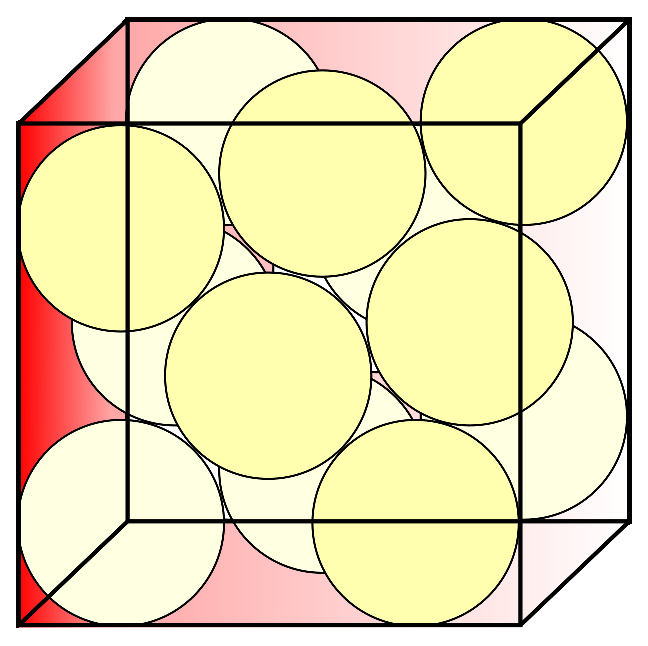
\includegraphics[width=0.5\textwidth]{nanospheres-cube.eps}
	\caption{Zero-dimensional nanocomposite structure. Nanoscale spheres are densely packed with a homogeneous host material filling the voids. A temperature gradient is shown, to illustrate use as a thermoelectric.}
	\label{fig:nanospheres-cube}
\end{figure}

\subsection{Investigation}
% Survey the paper, forward reference the interesting parts, make explicit your contributions to the problem
With the components discussed in the previous section, we have a clear plan of action. We must start by defining the non-equilibrium transport dynamics as in \secref{sec:boltz}. We then need a detailed description of phonons and electrons as is given in \secref{sec:phonons} and \secref{sec:electrical-transport}. Finally, we must apply these results to the EMA model and define the figure of merit ZT for our chosen nanocomposite structure, as is done in \secref{sec:ema} and \secref{sec:efficiency}. Our final results pull together all of this, to present a first principles theory of thermoelectric efficiency in a zero-dimensional SiGe nanocomposite.

\section{Background Theory}
\label{sec:background}
% Explain the intuition as if on a whiteboard
All the theories discussed in this report are transport processes. Therefore fundamental to them all are the non-equilibrium statistical mechanics of their quasiparticles.

\subsection{Boltzmann Equation}
\label{sec:boltz}
The Boltzmann equation describes the statistical behaviour of a thermodynamic system of particles not in thermodynamic equilibrium and its general definition is \cite{kittel}:

\begin{equation}
\label{eq:boltzmann-transport}
	\frac{f}{t} = \left(\frac{\partial f}{\partial
	t}\right)_\mathrm{force} + \left(\frac{\partial f}{\partial t}\right)_\mathrm{diff}+ \left(\frac{\partial f}{\partial t}\right)_\mathrm{coll}
\end{equation}

where $\frac{\partial f}{\partial t}$ is the time dependence of the distribution function of the particles $f$, the ``force" term represents external forces on the particles, the ``diff" term is the diffusion of particles through the system and the ``coll" term represents forces acting between particles in collisions.

From this general definition we can find how a particular system of particles or quasiparticles are distributed across a material and therefore find their average motion. We use this in the electrical conductivity $\sigma$ (\secref{sec:electrical-transport}) and phonon thermal conductivity $k_{ph}$ (\secref{sec:phonon-thermal}) derivations.

So we have a way of finding the distribution of our quasiparticles, but what exactly are the quasiparticles we are dealing with? And how are they important in the context of thermoelectrics?

\subsection{Phonons}
\label{sec:phonons}
A phonon is the quantisation of vibrational motion of a lattice of atoms at a single frequency, known as a normal mode \cite{kittel}. These phonons are quasiparticles, free to move around the crystal lattice and they are distributed according to the Bose-Einstein distribution \cite{kittel}:

\begin{equation}
\label{bose-einstein}
	 \bar{n} = \frac{1}{e^{(\hbar \omega) / k T} - 1}
\end{equation}

where $\bar{n}$ is the probability of a phonon existing with energy $\hbar \omega$ at temperature $T$. This distribution is shown in \figref{fig:3d-bose-einstein}

\begin{figure}
	\centering
	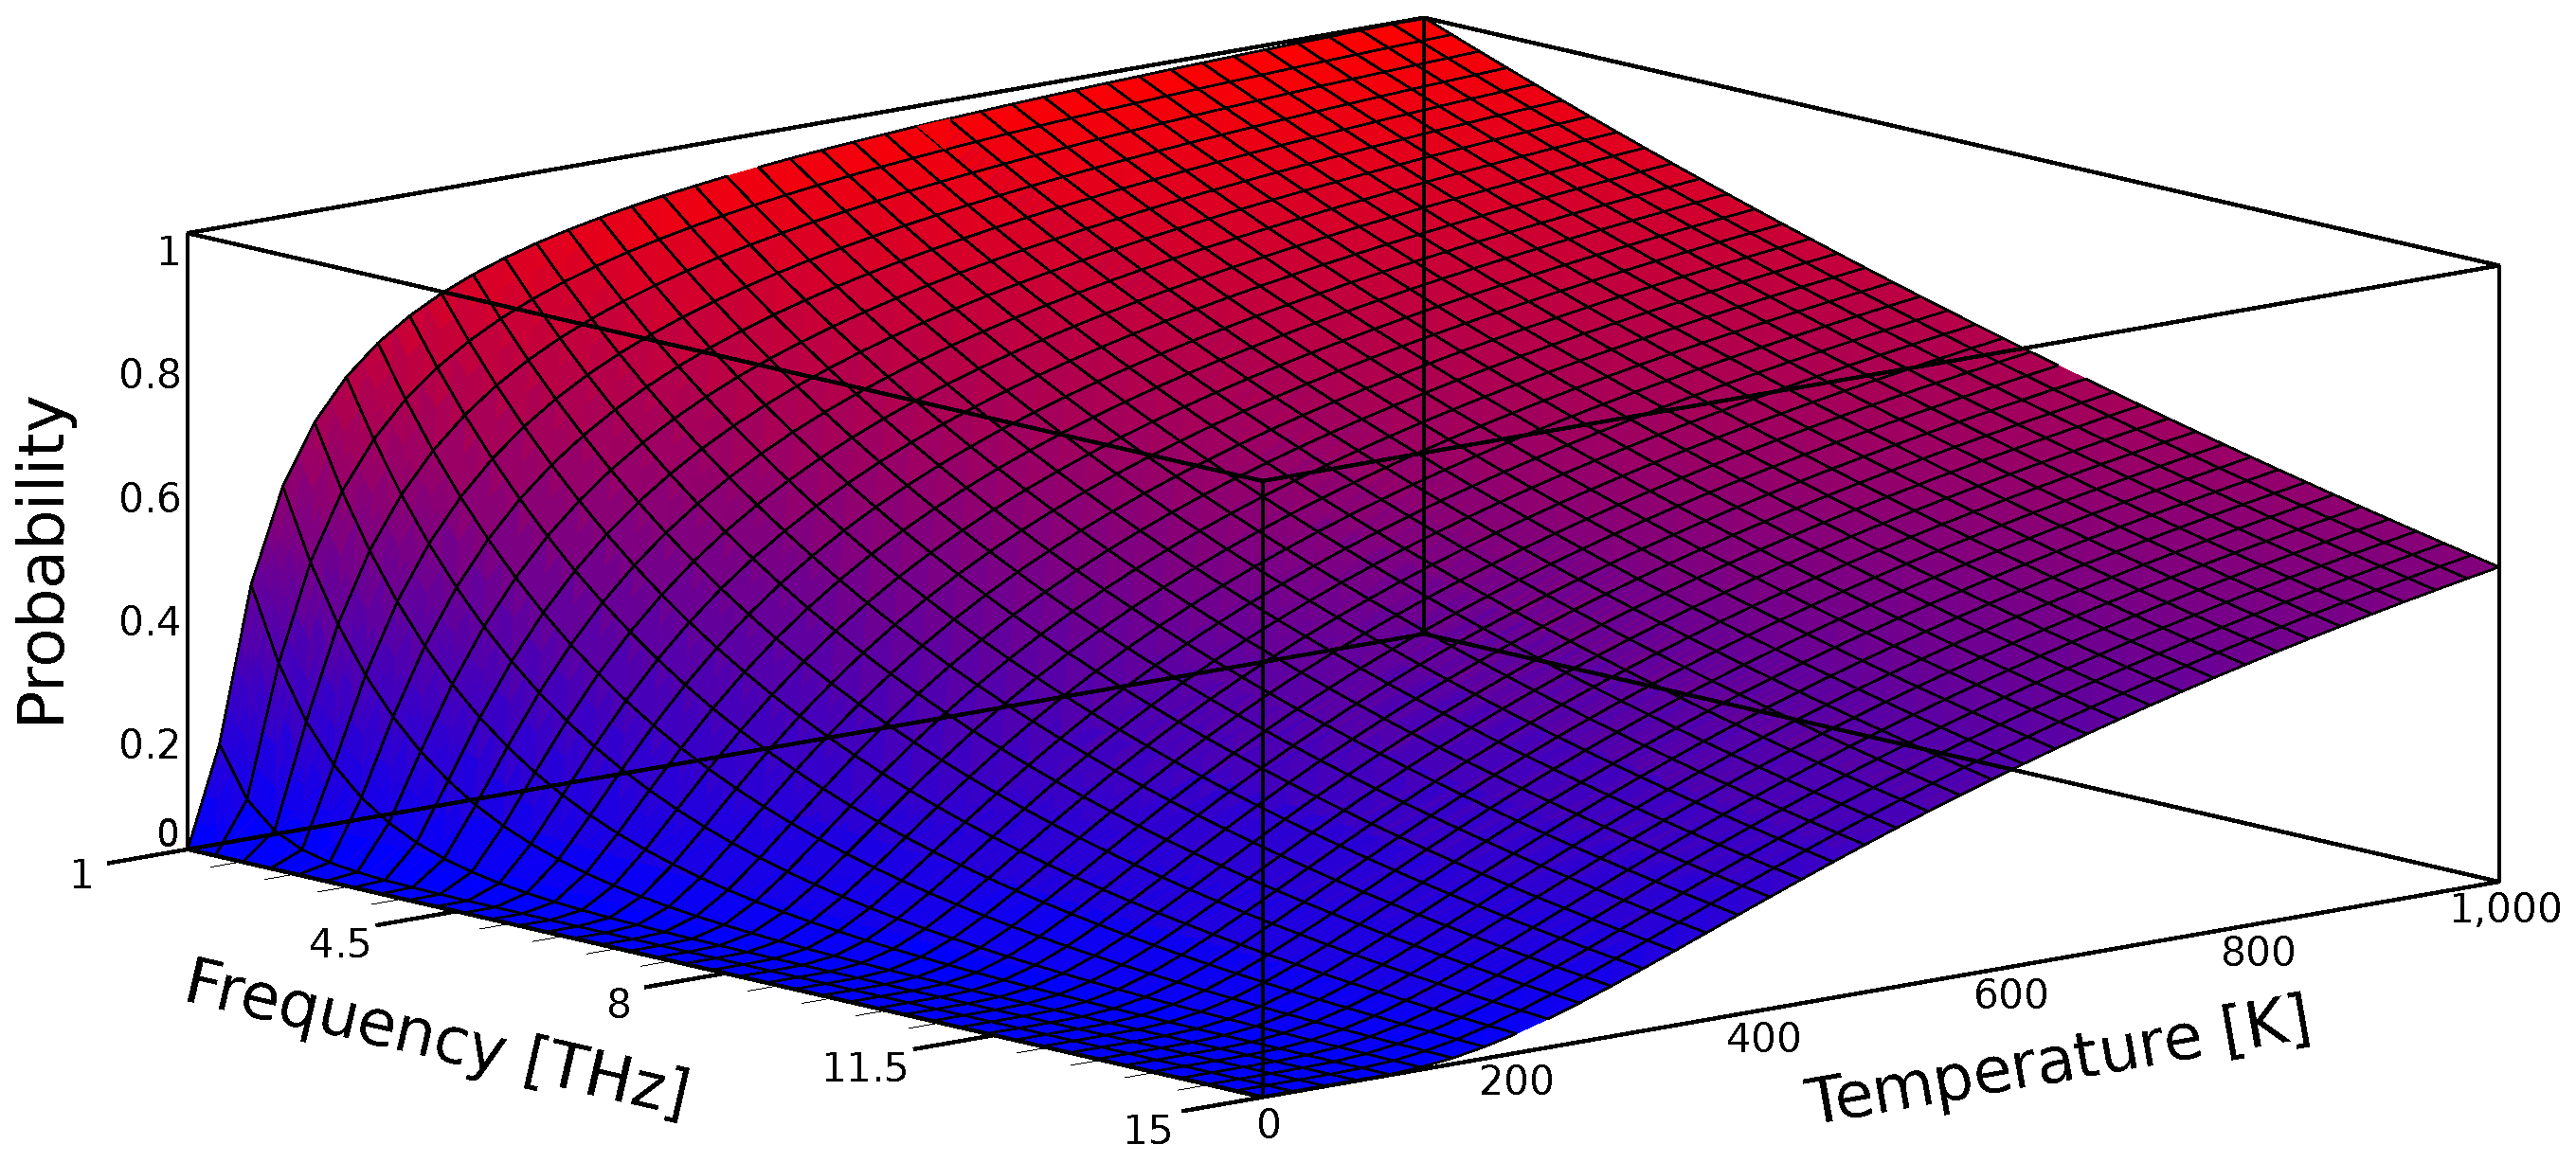
\includegraphics[width=\textwidth]{3d-bose-einstein.eps}
	\caption{Probability of phonon occupancy \emph{versus} phonon frequency and temperature, computed from the Bose-Einstein distribution \cite{kittel}. Frequencies at and above 15THz represent optical phonons.}
	\label{fig:3d-bose-einstein}
\end{figure}

Phonons are carriers of acoustic and thermal energy through a material. They follow two types of dispersion; optical and acoustic. These two dispersions are characterised by the type of atomic motion. For acoustic phonons there is coherent motion of the atoms out of their equilibrium positions. Whereas in optical phonons there is out of phase (incoherent) motion, one atom moving to the left, and its neighbour to the right. See \figref{fig:coherence-walk} for a visual depiction of coherence.

For typical thermal energies from room temperature to roughly the melting point of most semiconductors (~1300K), we can neglect the optical phonons. We can do this because the lower energy acoustic phonons are dominant. This is seen in the Bose-Einstein distribution \figref{fig:3d-bose-einstein}, where phonons with frequency at and above approximately 15THz are optical. There is a much higher probability for phonons at lower frequencies and therefore a much higher occupancy.

\begin{SCfigure}
	\centering
	\includegraphics[width=0.5\textwidth]{coherence-walk.png}
	\caption{An incoherent walk, contrasted with a coherent walk. For the coherent walk, the `atoms' keep step, they are in phase with their neighbours. For the incoherent walk, the `atoms' move in all directions, out of phase with each other.}
	\label{fig:coherence-walk}
\end{SCfigure}

\subsection{Debye Isotropic Continuum Model}
By assuming that we only have acoustic phonons, we are well justified in using the approximations in the Debye model, greatly simplifying the theory.

Our first approximation is that our nanocomposites form an \emph{isotropic continuum}, which means that the sample size is much larger than the typical phonon wavelength and it is the same everywhere. This is a valid assumption, as long as our nanocomposite structure is regular and periodic and we have macroscopic samples.

With this approximation, we can assume that our nanocomposite has translational symmetry. This enables us to invoke Bloch's theorem \cite{kittel}, which means for our phonons, all unit cells of the crystal lattice are equivalent. Mathematically this is $f(\vec{q}) = f(\vec{q} + \vec{T})$, where $\vec{q}$ is the wavevector and $\vec{T}$ is a lattice translation vector. The result of this is that if we can calculate properties for one unit cell, we have solved the entire crystal structure, momumentally simplfying the theory.

Our second approximation is that our unit cells can be modelled as a Debye spheres \cite{kittel}. This means that for a given unit cell, the wavevector $\vec{q}$ will be the same in all directions, forming a sphere. This is a good approximation, with a typical error of just 5-10\% \cite{gp}. Using we can easily derive the density of states, which can be used to calculate the specific heat, phonon mean free path and ultimately the phonon thermal conductivity.

\paragraph{Assumptions}
\begin{itemize}
  \item Optical phonons can be neglected up to 1300K
  \item Our nanocomposite structure is an isotropic continuum
  \item Unit cells can be modelled as Debye spheres
\end{itemize}

\subsection{Phonon Thermal Conductivity}
\label{sec:phonon-thermal}
Crucial to the EMA model \cite{ema} used in our nanocomposite theory, is the bulk phonon thermal conductivity $k_{ph}$. To find $k_{ph}$, we can model our phononic system as an ideal monatomic gas and use the kinetic theory of gases to describe their motion, leading to \cite{kittel}

\begin{equation}
\label{eq:phonon-thermal}
	k = \frac{1}{3} \int C(\omega) \nu(\omega) \Lambda (\omega) d\omega \approx \frac{1}{3}C\nu\Lambda
\end{equation}

where $C$ is the volumetric specific heat, $\nu$ is the phonon group velocity and $\Lambda$ is the phonon mean free path.

This can be derived more rigorously using the Boltzmann equation \eqref{eq:boltzmann-transport}. We can inspect a particular region of material, with $n$ as the number of phonons in this region. Phonons can leave this region by two mechanisms, \emph{diffusion} or \emph{decay}. Putting this together we get:

\begin{equation}
\label{eq:boltz-phonon-thermal}
	\frac{d \langle n \rangle}{dt} = \left(\frac{\partial \langle n \rangle}{\partial t}\right)_\mathrm{diffusion} + \left(\frac{\partial \langle n \rangle}{\partial t}\right)_\mathrm{decay}
\end{equation}

which, with some effort \cite{gp}, leads to:

\begin{equation}
\label{eq:phonon-thermal-rigor}
	k = \frac{1}{3} \sum_{\vec{q}, \vec{s}} C (\omega, \vec{s}) \nu (\omega, \vec{s}) \Lambda (\omega, \vec{s})
\end{equation}

where $\vec{q}$ and $\vec{s}$ are the wavevector and polarisation of the phonons.

We used the first expression \eqref{eq:phonon-thermal}, as an analytical approximation to the second expression \eqref{eq:phonon-thermal-rigor}. Using these analytical results as a guide, we numerically analysed the second expression \eqref{eq:phonon-thermal-rigor}. To use the first expression \eqref{eq:phonon-thermal} we must describe the phonons as a ideal monoatomic gas, so we make the following assumptions:
\paragraph{Assumptions}
\begin{itemize}
  \item The phonons are much smaller than the sample they exist in
  \item The phonons are numerous, so a statistical treatment can be used
  \item The phonons are in constant, random and rapid motion
  \item Phonon collisions are perfectly elastic.
  \item Other than collisions, there are no interactions between phonons
\end{itemize}

Surprisingly, despite these numerous assumptions, our numerical analysis of equation \eqref{eq:phonon-thermal-rigor} showed good agreement with the analytical results of equation \eqref{eq:phonon-thermal}. 

So we have derived an expression for $k$ and defined the parameters needed for phononic contribution to our thermoelectric nanocomposite. We must now derive the last pieces of the jigsaw; $\sigma$, $S$ and $k_{el}$.

An important quantity in defining $\sigma$, $S$ and $k_{el}$ is the Fermi level $E_F$. The Fermi level defines the highest occupied energy state of a system of electrons, at a given temperature $T$ \cite{kittel}. It is important in determining the number of electrons available for electrical conduction. So it's a good place to start the discussion.

\subsection{Fermi Level}
We are familiar with the derivation of the \emph{Fermi energy} \cite{kittel}, which is based upon Pauli's exclusion principle and defines the highest energy electron state at absolute zero. It is a relevant quantity in all materials for calculating solid state properties. However, with the small band gap of semiconductors used in thermoelectrics, additional temperature effects have to be accounted for.

The Fermi level for an intrinsic semiconductor can be defined as \cite{mckelvey}:

\begin{equation}
\label{eq:intrinsic-fermi}
	E_F = E_g + k_B T\ln\left(\frac{m^*_h}{m^*_e}\right)^\frac{3}{4}
\end{equation}

where $E_g$ is the band gap defined as $\frac{1}{2} (E_v + E_c)$, $E_v, E_c$ are the valence and conduction band edges and $m^*_e, m^*_h$ are the effective masses of electrons and holes.

For an extrinsic semiconductor the donor or acceptor atoms increase the Fermi level, but this is only significant at temperatures below a certain threshold. We must add an additional component to our intrinsic expression to account for this. This is well justified in McKelvey \cite{mckelvey}, for brevity I will simply state the new expression below:

\begin{equation}
\label{eq:extrinsic-fermi}
	E_F = E_g + k_B T\ln\left(\frac{m^*_h}{m^*_e}\right)^\frac{3}{4} + k_BT\sinh^{-1} \left(\frac{N_d-N_a}{2\sqrt{U_cU_v}e^{\frac{-E_g}{2k_BT}}}\right)
\end{equation}

where $N_d, N_a$ are the concentration of donor/acceptor atoms and $U_c, U_v$ are the effective density of states for the conduction/valence bands.

This expression is used in the derivation of all the electrical properties and it's the essential ingredient for the thermoelectric effect to be seen. See \figref{fig:fermi-level-compare} for a comparison plot between the extrinsic \eqref{eq:extrinsic-fermi} and intrinsic equations \eqref{eq:intrinsic-fermi} for an n-type SiGe semiconductor.

\paragraph{Assumptions}
\begin{itemize}
  \item The energy bands are parabolic and can be linearised at the band edges
  \item The effective masses of holes and electrons do not vary with temperature and can be resolved to a single parameter
  \item The density of donor or acceptor atoms does not change with temperature
\end{itemize}

\begin{figure}
	\centering
	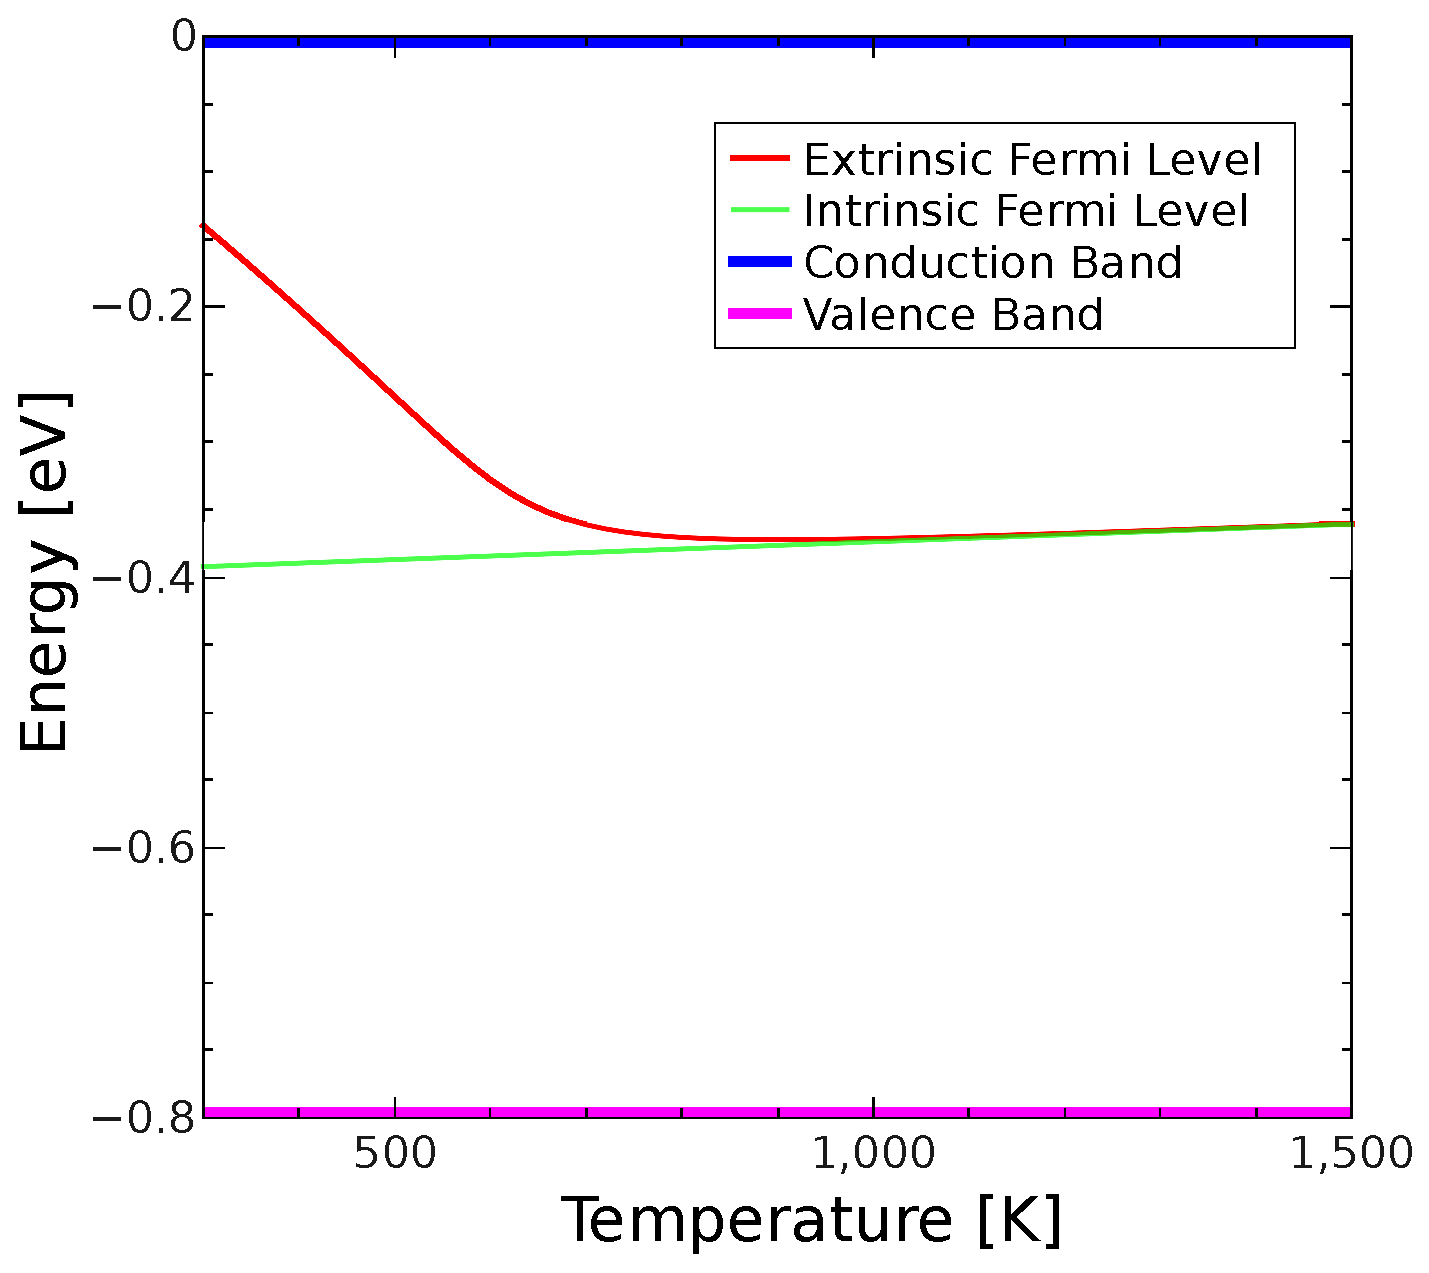
\includegraphics[width= \textwidth]{fermi-level-compare.eps}
	\caption{Extrinsic Fermi level \eqref{eq:extrinsic-fermi} and intrinsic Fermi level \eqref{eq:intrinsic-fermi} \emph{versus} energy for a n-type SiGe semiconductor. The extrinsic component of the Fermi level dominates over the intrinsic component from room temperature to 800K. Above 800K donor atoms have lost all their electrons and they no longer play a role in the Fermi level.}
	\label{fig:fermi-level-compare}
\end{figure}

\subsection{Electrical Transport}
\label{sec:electrical-transport}
The goal of our nanocomposite structuring is to enhance the heat to electric conversion efficiency and a vital component of that is the electrical conductivity $\sigma$. 

Kittel \cite{kittel} uses kinetic theory arguments similar to those in \secref{sec:phonon-thermal} to define a simple expression for electrical conductivity:

\begin{equation}
\label{eq:elec-cond}
	\sigma = n e \mu
\end{equation}

where $n$ is the number of charge carriers available for conduction, $e$ is the elementary charge and $\mu$ is the carrier mobility.

$n$ can be defined in terms of the density of states $g(\vec{q})$ and the distribution of charge carriers $f(\vec{q})$ as follows \cite{kittel}:

\begin{equation}
\label{eq:carrier-number}
	n = \int g(\vec{q}) f(\vec{q}) d\varepsilon = \frac{1}{6\pi^2} \left(\frac{2m_c k_B T}{\hbar^2}\right)^\frac{3}{2} F_\frac{1}{2}(\eta)
\end{equation}
where $\varepsilon$ is the energy range of interest, $m_c$ is the mass of the charge carrier, $T$ and $\eta$ is the reduced Fermi level equal to $\frac{E_f}{k_B T}$

This expression, along with a similar expression for mobility $\mu$ \cite{kittel} result in several non-analytical integrals called the \emph{Fermi-Dirac integrals}:

\begin{equation}
\label{eq:fermi-integral}
	F_r(\eta) = \exp(\eta) \int_0^\infty x^\eta \exp(-x) dx
\end{equation}

This can be approximated to $\exp(\eta)\Gamma(r+1)$ \cite{kittel}. It can also be evaluated numerically using a method such as Simpson's rule. We used both solutions throughout our project, implementing the extended Simpson's rule in Fortran for our final results.

Using the approximation above we arrive at a solution to the electrical conductivity equation \eqref{eq:elec-cond} is:

\begin{equation}
\label{eq:electrical-conductivity}
	\sigma = 2e (2\pi k_B T h^{-2})^\frac{3}{2} (m_e^* m_h^*)^\frac{3}{4} (\mu_e + \mu_h) \exp \left(\frac{-E_g}{2k_B T}\right)
\end{equation}

where $m_e^*, m_h^*$ are the effective masses of electrons and holes and $\mu_e, \mu_h$ are the mobilities of electrons and holes.

\section{Specific Theory}
% Details of exactly what you've done
% Tell a story, keep it concise, only explain what you need to
Now that we have the background theory we can understand the specific theories that apply to our zero-dimensional nanocomposite thermoelectric.
From a qualitative understanding, there must be strong boundary and interface effects; by definition nanocomposites contain numerous transitions between two or more materials, where each transition forms a new interface. Therefore a thorough understanding of how interfaces affect the propagation of phonons and electrons is required. However, we should first discuss the main topic of the project, thermoelectricity.

\subsection{Thermoelectricity}
In 1821, Thomas Seebeck discovered that circuit made from two dissimilar metals, with junctions at different temperatures would deflect a compass magnet (\figref{fig:seebeck-experiment}), he had discovered thermoelectricity. The temperature gradient $\vec{\nabla} T$ between the junctions generates an electromotive force:

\begin{equation}
\label{seebeck-emf}
	\vec{E_{emf}} = -S \vec{\nabla} T
\end{equation}

where $S$ is the Seebeck coefficient, defined as the induced voltage per unit temperature, mathematically $\Delta S = \frac{\Delta V}{\Delta T}$ \cite{modern-thermoelectrics}. A temperature gradient produces an electromotive force gradient, which in turn produces a current density gradient described macroscopically by a modified Ohm's law \cite{kittel}:

\begin{equation}
\label{current-density}
	\vec{J} = \sigma (-\vec{\nabla} V - S \vec{\nabla} T)
\end{equation}

where $\vec{J}$ and $\sigma$ are the current density $\frac{I}{A}$ and electrical conductivity at a given location in the material and $\vec{\nabla} T$ and $\vec{\nabla} V$ are the temperature and resultant voltage gradients across the material. If we were to repeat the experiment conducted by Seebeck (\figref{fig:seebeck-experiment}), but instead of a compass we use a voltmeter, we could find $\sigma$ and $V$. Assuming a steady state system, i.e. the current and current density are zero $I = \vec{J} = 0$, we could experimentally determine the Seebeck coefficient.

\begin{figure}
	\centering
	\includegraphics[width=\textwidth]{seebeck-experiment-black.png}
	\caption{Thomas Seebeck's original thermoelectricity experiment diagram \cite{seebeck-original}. A compass needle lies on top of one metal, underneath a bridge of a different metal (K), connected by two junctions and heated at one side. The heat produces a thermoelectric current in the junctions, creating a weak magnetic field, deflecting the compass needle.}
	\label{fig:seebeck-experiment}
\end{figure}

\subsection{Thermoelectric Efficiency}
\label{sec:efficiency}
The thermoelectric efficiency is best expressed in the dimensionless parameter $ZT$. The thermal efficiency $\eta$, is a function of $(ZT, T_h, T_c)$, where $Z$ is the figure of merit, $T = \frac{1}{2}(T_h + T_c)$, $T_h$ is the temperature at the hot junction and $T_c$ is the temperature at the cold junction. $ZT$ is defined as \cite{modern-thermoelectrics}:
\begin{equation}
\label{zt}
	ZT = \frac{S^2 \sigma T}{\kappa_e + \kappa_{ph}}
\end{equation}

where $S$ is the Seebeck coefficient from equation \eqref{seebeck-emf} \& \eqref{current-density}, $\sigma$ is electrical conductivity, $\kappa_e$ and $\kappa_{ph}$ are the thermal conductivity due to electrons and phonons respectively.

Important points to note about $ZT$ are that it is proportional to thermal efficiency $\eta$, is increased by a reduction in thermal conductivity and it depends on the square of the Seebeck coefficient. \figref{fig:zt-vs-doping} demonstrates the compromise between the variables in equation \eqref{zt}. $ZT$ values of current and previous generation thermoelectric materials have been plotted in \figref{zt-plot}.

\begin{figure}
	\centering
	\includegraphics[width=0.7\textwidth]{zt-temp-plot.png}
	\caption{Graph of thermoelectric figure of merit $ZT$ against temperature. The dashed line represents bulk thermoelectric materials, above the dashed line shows current generation nanocomposites \cite{minnich-review}.}
	\label{zt-plot}
\end{figure}

\subsection{Nanocomposites}

Composite materials are combinations of two or more materials, forming a new structure with significantly different physical or chemical properties than its constituent parts. In a similar way, nanocomposites are the structuring of multiple materials, but at the nanoscale. As our nanocomposites are at a comparable size to the crystal lattices of their constituent materials, we can view nanocomposites as artificial defects in a larger crystal lattice. A simple example of a 2D nanocomposite, a copper-graphene superlattice, is pictured in \figref{fig:superlattice} . Examining one layer of the superlattice, the material in bulk form would be a 3D crystal structure, but by constraining the layer thickness we have introduced a boundary defect. The periodic array of these boundary defects forms a new 3D artificial crystal, which we define as a superlattice, a nanocomposite.

\begin{figure}
	\centering
	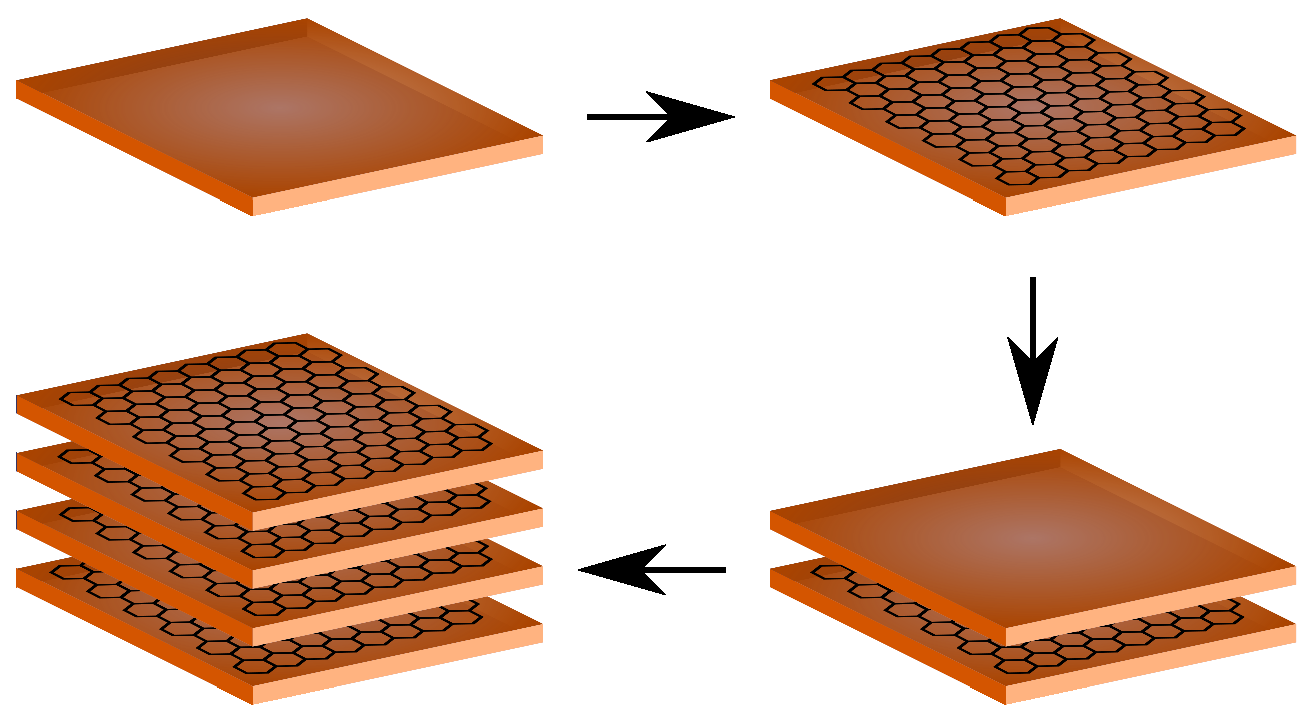
\includegraphics[width=0.7\textwidth]{graphene-superlattice.eps}
	\caption{Superlattice of graphene and copper. Alternate layers of nanoscale copper and graphene are sandwiched together to form a new 3D artificial crystal, with distinct properties.}
	\label{fig:superlattice}
\end{figure}

There are several other possible nanocomposite structures. The most common are depicted in \figref{fig:nanocomposite-structures}.

\begin{figure}
	\centering
	\includegraphics[width=\textwidth]{nanocomposite-structures.png}
	\caption{A range of possible nanocomposite structures, arranged in increasing dimensionality. Our chosen system is a \emph{composite nanoparticle} \cite{nanowires}.}
	\label{fig:nanocomposite-structures}
\end{figure}

There has been experimental progress in the field of nanocomposites, structures such as the ones seen in \figref{fig:nanopillars} have been created.

\begin{figure}
	\centering
	\includegraphics[width=0.8\textwidth]{stem-pillar-composites-edit.pdf}
	\caption{A recently fabricated 3D nancomposite structure \cite{minnich-review}.}
	\label{fig:nanopillars}
\end{figure}


\subsection{Effective Medium Approximation}
\label{sec:ema}
The effective medium approximation (EMA) considers a homogeneous host material with a phonon thermal conductivity $k_h$, that is regularly perturbed by an interface resistance $R$ and separate phonon thermal conductivity $k_p$, which is then averaged over a relevant length scale $d$. For spherical particles the theory takes the following form \cite{ema}:

\begin{equation}
\label{eq:ema}
	\frac{k_e}{k_h} = \frac{k_p (1 + 2\alpha) + 2k_h + 2	\varphi [k_p (1 - \alpha) - k_h]}{k_p (1 + 2\alpha) + 2k_h -	\varphi [k_p (1 - \alpha) - k_h]}
\end{equation}

where $k_e$ is the effective composite thermal conductivity, $k_h$ is the host material thermal conductivity, $k_p$ is the particle thermal conductivity, $\varphi$  is the volume fraction of nanoparticle inclusions and $\alpha = R / (d / 2)$, where $R$ is the thermal boundary resistance and $d$ is the diameter of the spherical particles.

The crucial problem with this theory in application to nanocomposites, is that it fails to account for the increased scattering in and around particles. The modified-EMA (mEMA) \cite{mema} introduces additional terms into the mean free path of the thermal conductivity expressions to address the issue:

\begin{equation}
\label{eq:mema}
	\Lambda_{\textsc{coll}} = \frac {4a^3}{\pi d^2}
\end{equation}

where $a$ is the unit cell effective length defined from the density of nanoparticles $n = 1 / a^3$, $d$ is the diameter of the nanoparticles.

Using this in the equations derived for phonon thermal conductivity in \secref{sec:phonon-thermal}, we can define a new effective $k_p$ and $k_e$, which we then substitute back into \eqref{eq:ema}. This additional scattering is significant and it substantially lowers the phonon thermal conductivity.

Studying the mEMA closer, we found that the smallest possible particles would give the lowest phonon thermal conductivity. We decided upon 10nm as our final particle size, as it is comparable with the phonon wavelength. If used smaller particles, then the idea of a phonon breaks down.

\section{Results and Analysis}
% Split into two sections if lengthy
% Explain all elements leading to the results
% Include key graphs, have minimal tables
% What do they show?

To get our final results, we computed each component of the ZT expression \eqref{zt} in Fortran, using materials data from Springer \cite{springer}. We used the extended Simpson's rule to compute any integrals and solved what we could analytically. We took a nanocomposite of 10nm silicon spheres, at near maximum filling, which roughly corresponds to a ratio of 70-30 GeSi.

\figref{fig:mEMA-temp-10nm-log} compares 4 different nanocomposite phonon thermal conductivity models. It shows the progressive decrease in phonon thermal conductivity, as more nanostructuring effects are considered. The \emph{specularity EMA} is not mentioned in the report, since the derivation was lengthy and it did not produce significantly different results from the mEMA.

%\figref{fig:all-in-one} plots all of the different electrical transport properties on one graph, to show how their temperature dependence. Our results all gave negative slopes to the electrical properties, which is in agreement with what we would expect.

EMA models show a surprisingly constant temperature dependence. This is likely because of the dominance of diffuse phonon scattering at particle interfaces. From our analysis, it is clear that maximising the particles surface area per unit volume (interface density) is key to minimising the phonon thermal conductivity. It appears to have no effect on the electrical transport properties, thus at 0.3 volume fraction, a 10$\times$ increase in ZT could potentially be realised.

\figref{fig:zt-10nm} shows the final ZT values for our nanocomposite structure. Comparing this to \figref{zt-plot}, we can see that over the usable temperature range of 700-1200K, the nanostructuring has increased ZT roughly 4$\times$. The primary mechanism for this is likely to be scattering in between nanoparticles, but further investigation is required.

\begin{figure}
	\centering
	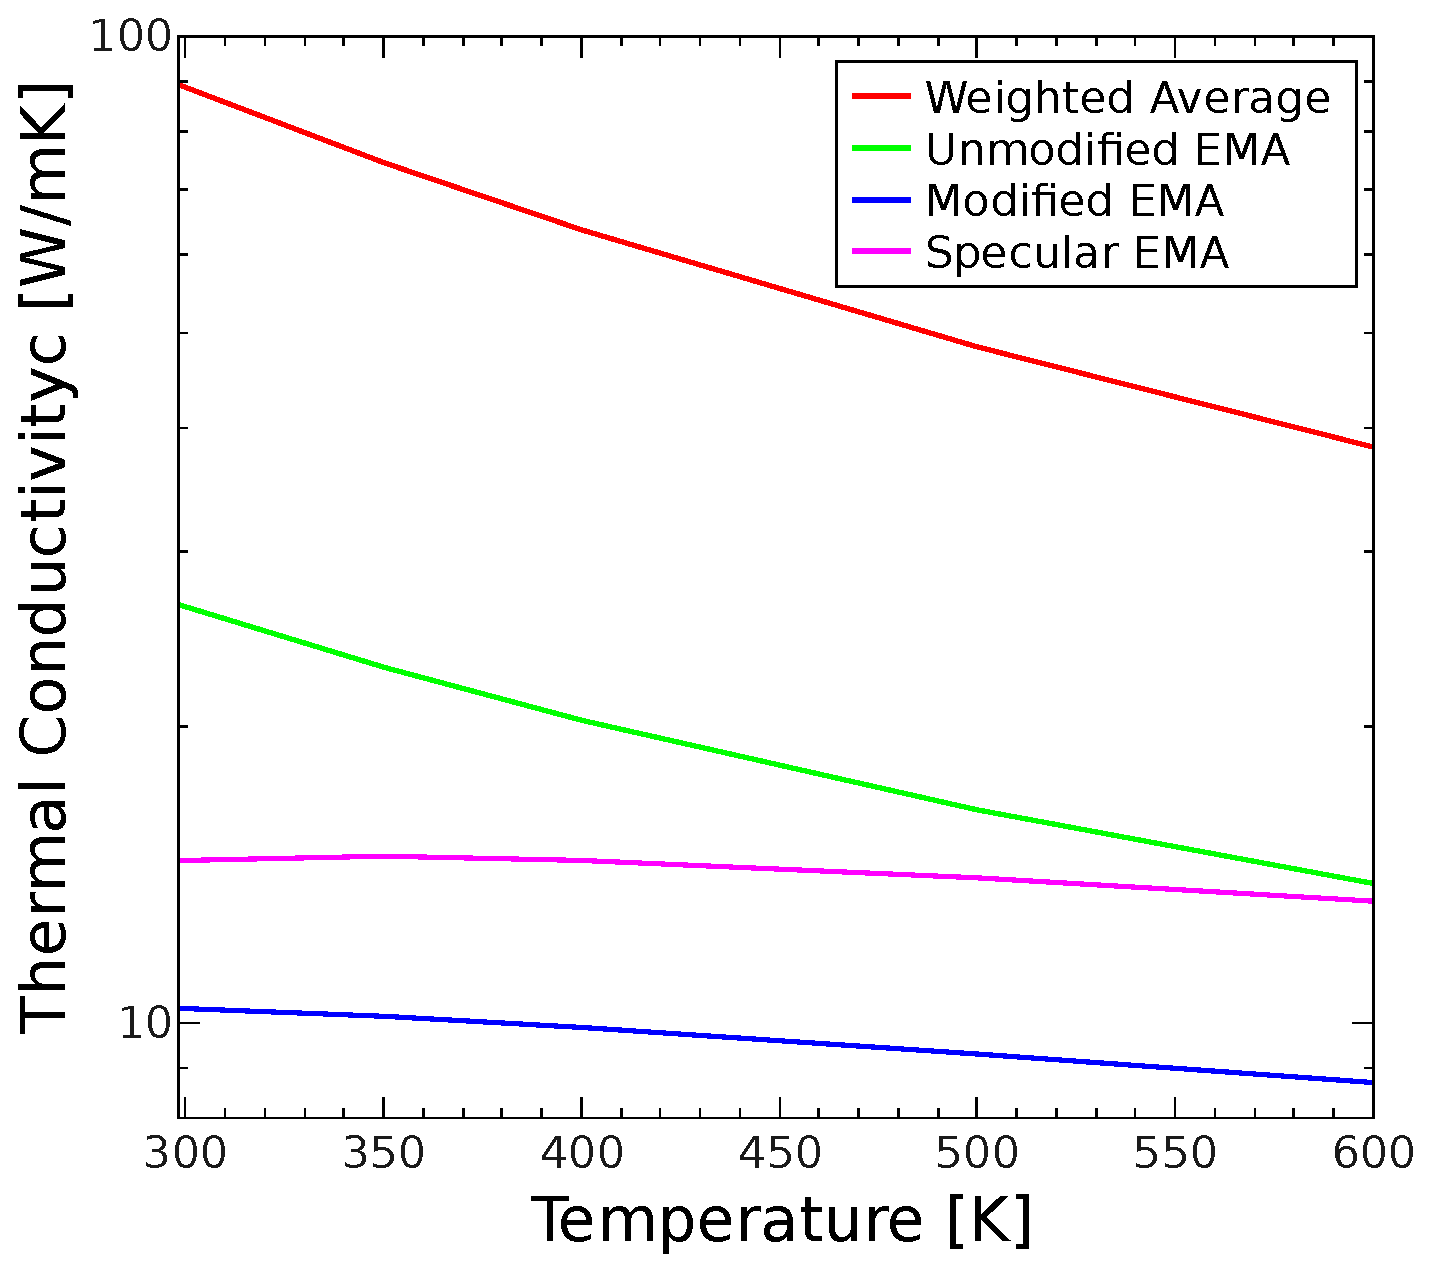
\includegraphics[width=0.8\textwidth]{mEMA-temp-10nm-log.eps}
	\caption{A comparison between 4 different nanocomposite $k_ph$ models. 0.1 volume fraction corresponds to 90\% Ge, 10\% Si. Each model considers progressively smaller size scales with more detail.}
	\label{fig:mEMA-temp-10nm-log}
\end{figure}

\begin{figure}
	\centering
	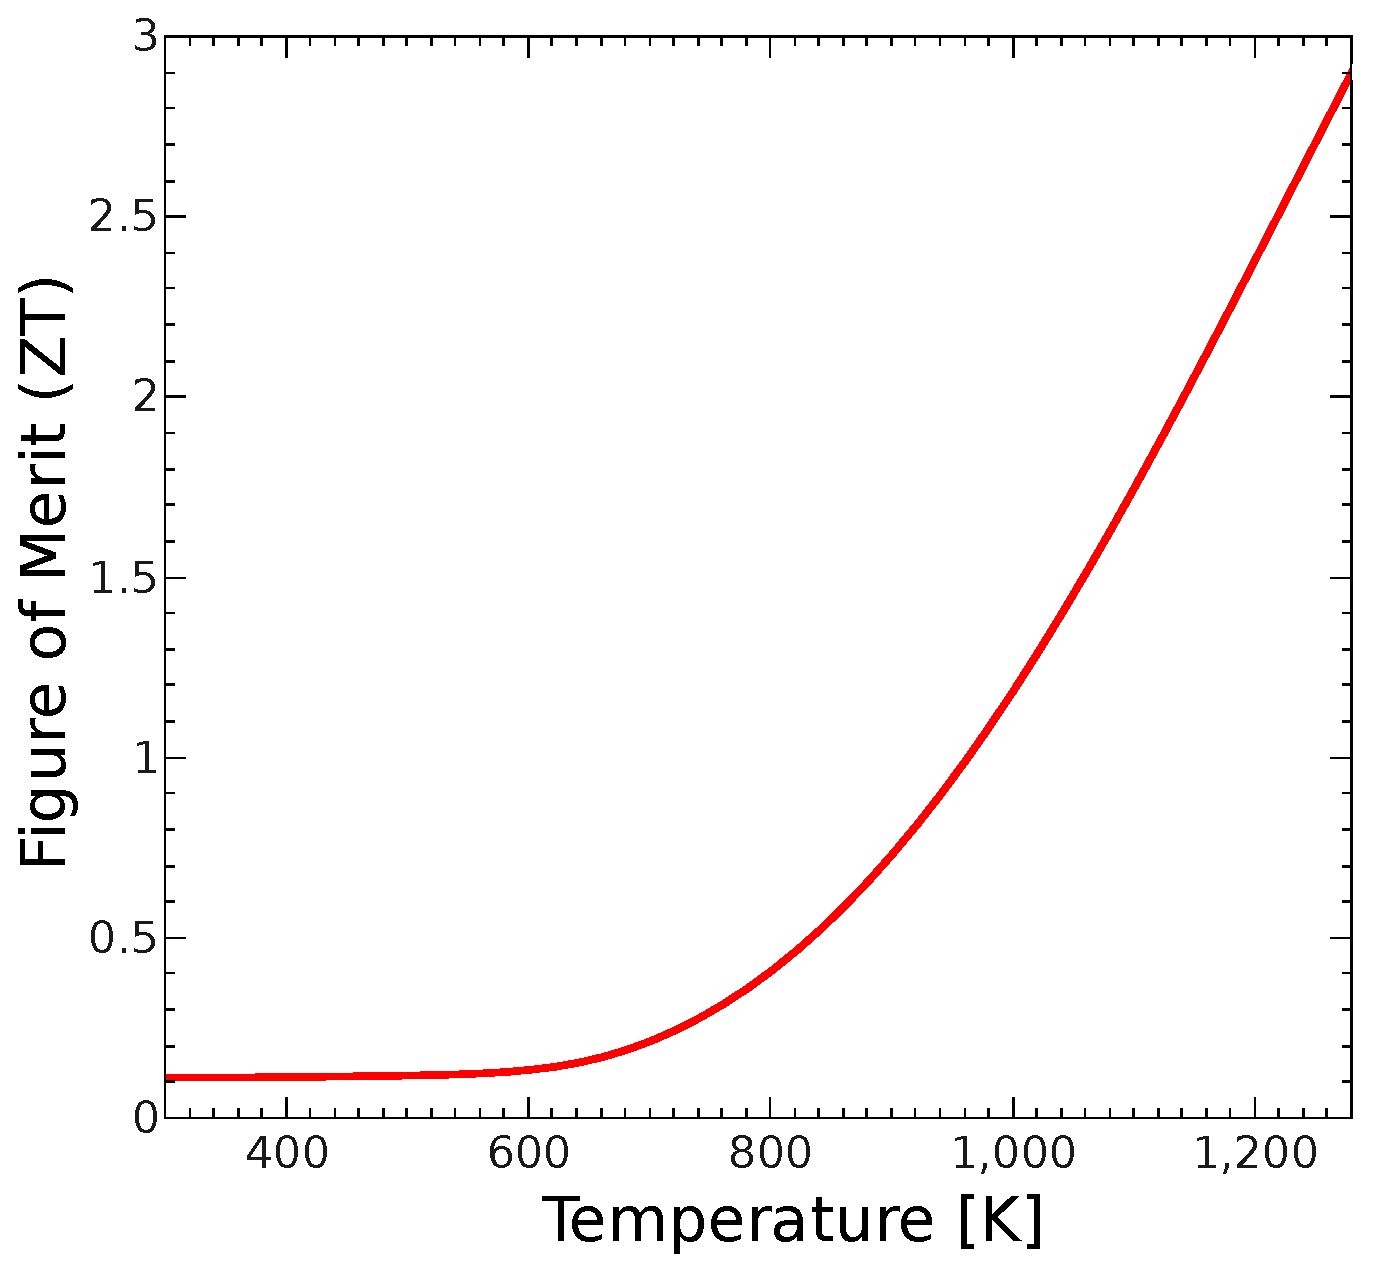
\includegraphics[width=\textwidth]{ZT-10nm.eps}
	\caption{ZT \emph{versus} temperature for a 70-30 GeSi zero-dimensional nanocomposite. As temperature increases, the decreasing thermal conductivity, greatly enhances ZT. Comparing to \figref{zt-plot} we see that ZT has increased roughly 4$\times$ over the usable temperature range (700-1200K).}
	\label{fig:zt-10nm}
\end{figure}

\section{Conclusion and Future Work}
% Summarise results
% What else could be done?
We have derived expressions for the electrical and thermal conductivities of a 10nm 30-70 SiGe nanocomposite. We utilised an effective medium approximation to calculate phonon thermal conductivity and find that nanostructuring greatly reduces this quantity. We find that phonon thermal conductivity is minimised for silicon spheres of up to 10nm diameter. Further investigation may find that smaller spheres are possible and give an even greater decrease in the phonon thermal conductivity.

With our analysis we find that nanocomposite structuring increases the thermoelectric efficiency approximately 4$\times$ compared to bulk SiGe. This gives good indication that further theoretical and experimental research should be conducted in this field.

\subsection{Future Work}
\begin{itemize}
  \item Create a nanocomposite theory of electrical transport
  \item Find temperature dependent material properties (band gap etc.) and calculate ZT
  \item Derive an expression for the total efficiency of a thermoelectric generator. Is the ZT improvement translatable to a real world application?
  \item Investigate the effects of non-spherical particle shapes. Particularly a tessellating 3D shape, to maximise interface density
  \item Derive a non-phonon based theory to investigate nanoparticle sizes smaller than 10nm
\end{itemize}

% Link to your online repository
\subsection{Online repository}
\url{https://github.com/kahlos/thermoelectrics}

\pagebreak

% The {number} is related to the number of digits required for the references
\begin{thebibliography}{11}

\bibitem{modern-thermoelectrics}
D. M. Rowe,
\emph{Modern Thermoelectrics},
September 1983,
Holt-Technology,
ISBN:978-0835945936
\textbf{Page 12}

\bibitem{engine-efficiency}
M. L. Baglione,
\emph{Development of System Analysis Methodologies and Tools for Modeling and Optimizing Vehicle System Efficiency},
2007,
University of Michigan,
DOI:2027.42/57640
\textbf{Pages 52-54}

\bibitem{nanocomposite-zt}
R. Venkatasubramanian \emph{et al.},
\emph{Thin-film thermoelectric devices with high room-temperature figures of merit},
October 2001,
Nature, vol. 413, pp. 597-602,
DOI:10.1038/35098012

\bibitem{liu-review}
W. Liu \emph{et al.},
\emph{Recent advances in thermoelectric nanocomposites},
January 2012,
Nano Energy, vol. 1, iss. 1, pp. 42-56,
DOI:10.1016/j.nanoen.2011.10.001

\bibitem{solar-thermal}
D. Kraemer \emph{et al.},
\emph{High-performance flat-panel solar thermoelectric
generators with high thermal concentration},
May 2011,
Nature Materials 10, pp. 532-538,
DOI:10.1038/NMAT3013

\bibitem{exhust-recovery}
X. Liu \emph{et al.},
\emph{A case study on compatibility of automotive exhaust thermoelectric generation system, catalytic converter and muffler},
March 2014,
Case Studies in Thermal Engineering, vol. 2, pp. 62-66,
DOI:10.1016/j.csite.2014.01.002

\bibitem{thermo-cooling}
L. E. Bell,
\emph{Cooling, Heating, Generating Power, and Recovering Waste Heat with Thermoelectric Systems},
September 2008,
Science 12, vol. 321, no. 5895, pp. 1457-1461,
DOI:10.1126/science.1158899

\bibitem{minnich-review}
A. J. Minnich \emph{et al.},
\emph{Bulk nanostructured thermoelectric materials: current research and future prospects},
Feburary 2009,
Energy Environ. Sci. 2, pp. 466-479,
DOI:10.1039/B822664B

\bibitem{crc-handbook}
G. A. Slack, ed. D. M. Rowe,
\emph{CRC Handbook of Thermoelectrics},
1995,
CRC Press,
ISBN:978-0849301469
\textbf{Pages 407-440}

\bibitem{nanowires}
L. D. Hicks, M. S. Dresselhaus,
\emph{Thermoelectric figure of merit of a one-dimensional conductor},
June 1993,
Phys. Rev. B 47, 16631
DOI:10.1103/PhysRevB.47.16631

\bibitem{ema}
C. Nan \emph{et al.},
\emph{Effective thermal conductivity of particulate composites with interfacial thermal resistance},
February 1997,
Journal of Applied Physics 81, pp. 6692-6699,
DOI:10.1063/1.365209

\bibitem{phm}
L. Braginsky \emph{et al.},
\emph{High-temperature phonon thermal conductivity of nanostructures},
October 2002,
Physical Review B 66, 134203,
DOI:10.1103/PhysRevB.66.134203

\bibitem{kittel}
C. Kittel,
\emph{Introduction to Solid State Physics}, 8th Ed.,
November 2004,
John Wiley \& Sons,
ISBN:978-0471415268

\bibitem{gp}
G.P Srivastava,
\emph{The Physics of Phonons},
January 1990,
CRC Press,
ISBN:978-0852741535

\bibitem{mckelvey}
J. P. McKelvey,
\emph{Solid State and Semiconductor Physics},
1966,
Harper \& Row,
ISBN:978-0898743968
\textbf{Pages 109-111}

\bibitem{seebeck-original}
\url{etc.usf.edu/clipart/35600/35659/seebeck_35659_lg.gif},
24 November 2013

\bibitem{mema}
A. Minnich, G. Chen,
\emph{Modified effective medium formulation for the thermal conductivity of nanocomposites},
August 2007,
Appl. Phys. Lett. 91, 073105,
DOI:10.1063/1.2771040

\bibitem{springer}
Springer,
\emph{Springer Handbook of Condensed Matter and Materials Data},
2005,
ISBN: 978-3540443766

\end{thebibliography}

\pagebreak

\appendix

\begin{center}
{\Huge\textbf{Appendix}}
\end{center}

%\section{Further Questions and Thoughts}

%\section{List of Assumptions}

%\section{Further Reading}

\section{Tools and Software}

\begin{itemize}
  \item Github - An online version control repository
  \item QtiPlot - Plotting graphs and quick checks of results
  \item Fortran - Programming computational analysis
  \item LaTeX - Typesetting this document
\end{itemize}

\section{Physical Data}
All physical constants used were from the CODATA Recommended Values of the Fundamental Physical Constants [2010] \url{physics.nist.gov/Constants}

All materials data were sourced from the \emph{Springer Handbook of Condensed Matter and Materials Data} \cite{springer}

%\section{Program Code}

\end{document}


